\documentclass[a4paper,12pt]{article}
\usepackage{mathtools,amsfonts,amssymb,amsmath, bm,commath,multicol}
\usepackage{algorithmicx, tkz-graph, algorithm, fancyhdr, pgfplots}
\usepackage{fancyvrb}

\usepackage[noend]{algpseudocode}

\pagestyle{fancy}
\fancyhf{}
\rhead{3/5/2017 ::: Nandan Rao}
\lhead{Social and Economic Networks ::: Problemset 1}
\rfoot{\thepage}


\DefineVerbatimEnvironment{juliaout}{Verbatim}{}
\DefineVerbatimEnvironment{juliacode}{Verbatim}{fontshape=sl, fontsize=\tiny}
\DefineVerbatimEnvironment{juliaterm}{Verbatim}{}


\begin{document}


\section*{Barabasi}

\subsubsection*{Matrix Formalism}

The matrix times the one vector will give the degree count:
$$
A1
$$

Total number of links:
$$
\frac{(A 1)^T1 }{2}
$$

Number of triangles present (anyone whose second neighbor is themself!):
$$
Tr(A^3)\frac{1}{6}
$$

Sum of nodes neighbors:
$$
A^2 1
$$

Sum of nodes second neighbors:
$$
A^3 1
$$

\subsubsection*{Bipartite Networks}

Every adjacency matrix will have zero on the diagonal. The bipartite version exapnds those zeros because not only will 1 not be connected to 1, it won't be connected to anything on its side, which is 1 all the way to 7 in this case!

<<>>=
b_edges = [0 0 0 0 0 0 1 0 0 0 0
           0 0 0 0 0 0 0 0 1 0 0
           0 0 0 0 0 0 1 1 1 0 0
           0 0 0 0 0 0 0 0 1 1 0
           0 0 0 0 0 0 0 0 1 0 1
           0 0 0 0 0 0 0 0 0 0 1
           1 0 1 0 0 0 0 0 0 0 0
           0 0 1 0 0 0 0 0 0 0 0
           0 1 1 1 1 0 0 0 0 0 0
           0 0 0 1 0 0 0 0 0 0 0
           0 0 0 0 1 1 0 0 0 0 0]
@
Average degree of purple:
$$
\frac{1 + 1 + 3 + 2 + 2 + 1}{6} = 1.667
$$

Average degree of green:
$$
\frac{2 + 1 + 4 + 1 + 2}{5} = 2
$$

Average degree in projections purple:
$$
\frac{1 + 3 + 3 + 3 + 4 + 1}{6} = 2.5
$$

Average degree in projections green:
$$
\frac{2 + 2 + 4 + 1 + 1}{5} = 2.4
$$

The averages obtained separately are different in the same way that more inclusive measurements of centrality will be different from that obtained by simply counting the degree of the node. In this case, we are calculating, in a sense, the 2-neighborhood centrality of the node, which will naturally different from the 1-neighborhood!

\subsubsection*{Bipartite Networks - General Considerations}

The maximum number of links a bipartite graph can have is:
$$
N_1N_2
$$
Compared to a non-bipartite graph with the same number of nodes:
$$
diff = (N_1 + N_2)(N_1 + N_2 - 1) - N_1N_2
$$

Given $N_1 << N_2$, as $N_1$ shrinks, the maximum possible links in a non-bipartite graph gets close to the square of $N_2$ and further from $N_2N_1$, therefore the ratio heads towards zero.
%
The average degree is naturally correlated with the number of nodes in the opposite set, if the probability of connection is independent of those numbers.


\section*{Easley and Kleinberg 14.6}

\subsubsection*{a}
Naturally all nodes with the same letter have the same value, after the first round this is:

A:9, B:27, C:5, D:25

\subsubsection*{b}



\subsubsection*{c}
The intuition says that the A hubs and B authorities should converge to a much higher value than the C hubs and D authority. This can be seen mathematically most clearly in the step of counting the hub values, which will go up faster for the A hubs as they have more B authorities they are connected to!

\section*{Problem 1}

\subsubsection*{a}

<<warning=false;echo=false>>=
using LightGraphs
using GraphPlot
using Gadfly

edges = [0 1 1 0 0 0 0 0 0 0
         1 0 1 0 0 0 0 0 0 0
         1 1 0 1 1 0 0 0 0 0
         0 0 1 0 0 0 0 0 0 0
         0 0 1 0 0 1 1 1 1 0
         0 0 0 0 1 0 0 0 0 0
         0 0 0 0 1 0 0 0 0 1
         0 0 0 0 1 0 0 0 0 1
         0 0 0 0 1 0 0 0 0 1
         0 0 0 0 0 0 1 1 1 0]


g = Graph(edges)
@

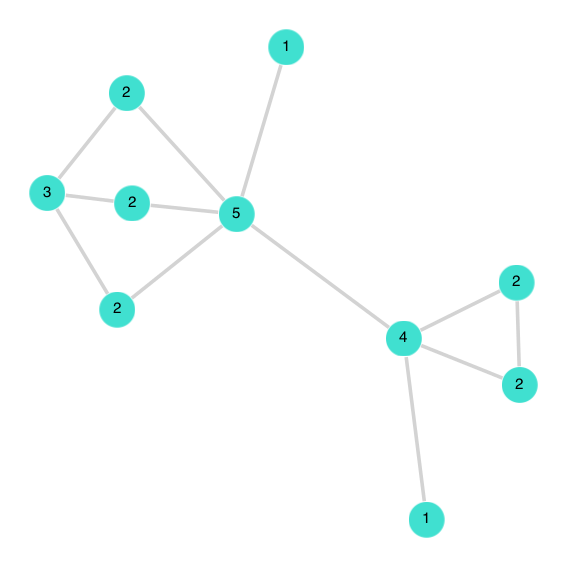
\includegraphics[width=\linewidth]{figures/labels.png}

<<warning=false;echo=false>>=
plot(x = degree(g), Geom.histogram)
@

\subsubsection*{b}

The average clustering is simply:

$$
\frac{1 + 1 + \frac{1}{6}}{10} = \frac{13}{60}
$$

The local clustering is as follows, it's fairly minimal in this graph because so many nodes are stars!

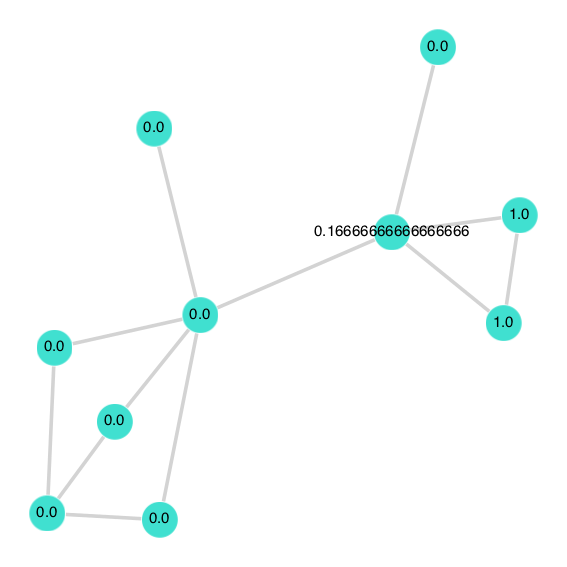
\includegraphics[width=\linewidth]{figures/clustering.png}

\subsubsection*{c}

Diameter is 4. The average distance, averaging over the off-diagonal elements of the distance matrix, is approximately 2.1778.


\section*{Problem 2}

\subsubsection*{a.1}
<<warning=false;echo=false>>=
plot(xmin = [0.5, 3.5], xmax = [1.5, 4.5], y = [3, 1], Geom.bar)
@

\subsubsection*{a.2}
Diameter is 2 and average distance is 1.6.

\subsubsection*{a.3}

\subsubsection*{b.1}
If 2-regular graph is a circle!!! If the graph is connected, there is only one graph that is n=9 and k=2 regular.

\subsubsection*{b.2}


\subsubsection*{c.1}
The first is not, as a triangle can never be part of a bipartite graph. The second is, the same logic as the circle graph below, just in two dimensions (start with one node, put it in one set, put its neighbors in the other, continue to its neighbors and do the same, and you will collect all the nodes into two distinct sets).

\subsubsection*{c.2}
A star is bipartite by definition, with the central node in one set, and all the others in the other set. A circle graph, is only bipartite if it has an even number of nodes, in which case every second node is in one set, with the remain in the other.



\section*{Problem 3}
The node with the highest closeness centrality, in an undirected graph such as this one, will be the node that is quickest to get to from every other node in the graph. Closeness centrality measures the distance of travel necessary to reach EVERY other node in the network from the node in question. It does this by simply summing up the distance and inverting that number, and you can normalize by the total number of nodes if you need to compare between networks.

In this situation we can think of measuring closeness centrality by dropping a single worker in each node, make them walk to work, then pay them each a euro for every km walked. The node with the highest closeness centrality is the node that minimizes our cost.

This simple measure is ideally suited to situation two. Not knowing how many people live at each node, we are forced to weight each node equally, which closeness centrality does explicitly. In situation one, we might use closeness centrality as lacking information about the distance of each edge, we are forced to assume each edge has an equal distance, and closeness centrality will also give us the point that minimizes the total distance traveled with one worker per node and one euro per edge.

In situation three, however, closeness centrality in its most basic form will not suit us. If we stick to our example of the worker that we pay one euro per kilometer walked, what we need instead is to simply drop the number of workers at each node proportional to the number of residents of that node. So for each node we multiply the distance by the number of people living in that node, and again choose the node that minimizes that cost (maximizes the inverse, or the closeness).

\end{document}